\documentclass{article}
\usepackage{multirow}
\usepackage{wrapfig}
\usepackage{graphicx}
\usepackage{hyperref}
\hypersetup{
    colorlinks=true,
    linkcolor=blue,
    filecolor=magenta,      
    urlcolor=blue,
    }
\title{LaTeX Workshop}
\author{Oscar Tuff}
\date{\today}

\begin{document}
\maketitle
\tableofcontents
\newpage
\section{exercise 1:}
\begin{center}
	\begin{tabular}{ |c|c|c| }
		\hline
		cell1 & cell2 & cell3yeet \\
		cell4 & cell5 & cell6     \\
		cell7 & cell8 & cell9     \\
		\hline
	\end{tabular}
\end{center}

\section{exercise 2:}
\begin{wrapfigure}{r}{0.5\textwidth}
	\vspace{-30pt}
	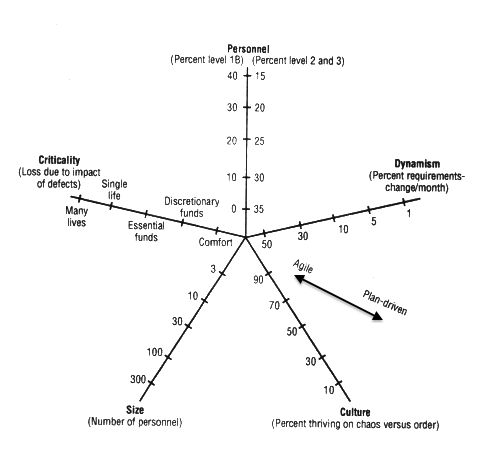
\includegraphics[width=0.48\textwidth]{boehmturner}
	\caption{Boehm-Turner model}
\end{wrapfigure}
text wrapping the picture ....
\\
\\
\\
\\
\\
\\
text \cite{lamport94}
\\
\\
\\
\\
\section{exercise 3:}
text \cite{texbook}
\\
\url{https://www.overleaf.com/learn/latex/Bibliography_management_with_bibtex}

\begin{thebibliography}{99}
	\bibitem{texbook}
	Donald E. Knuth (1986) \emph{The \TeX{} Book}, Addison-Wesley Professional.

	\bibitem{lamport94}
	Leslie Lamport (1994) \emph{\LaTeX: a document preparation system}, Addison Wesley, Massachusetts, 2nd ed.
\end{thebibliography}

\section{exercise 4:}
\url{https://www.overleaf.com/learn/latex/Multi-file_LaTeX_projects}

moretext
\section{exercise 5:}
moretext
\section{exercise 6:}
moretext
\section{exercise 7:}
moretext
\end{document}
